\chapter{High-Throughput Satellite Communication Systems}
\label{chapter:hts_communication_systems}

The preceding chapters developed the theory of linear precoding for generic \ac{SU}- and \ac{MU}-\ac{MIMO} systems. Before turning to the specific problem addressed by this work, the present chapter situates these results within the context of satellite communications.
We first motivate the use of precoding in modern \acf{HTS} systems and describe the system architecture considered in the remainder of this work. We then discuss the channel features and modeling assumptions that distinguish the satellite setting from the terrestrial \ac{MU}-\ac{MIMO} scenario of Chapter~\ref{chapter:mu_mimo_precoding}. Finally, we review the main families of precoding techniques proposed in the literature and identify the specific category that is relevant for our work.


\section{Motivation}
\label{section:hts_motivation}
% ==========================
%       Motivation
% ==========================

% importance of satellite communications
Satellite communications have recently regained considerable attention as a key enabler of ubiquitous broadband connectivity. 
They provide cost-efficient coverage of large geographical areas, including regions where deploying a terrestrial infrastructure is impractical, and are envisioned as an integral component of future 5G and beyond networks~\cite{1_signal_processing_for_satellites, 6_satellites_in_new_space_era}.

% interference -> precoding
To meet the rapidly growing demand for data rates, modern satellite systems have evolved from single-beam architectures toward \acf{HTS} systems, in which the coverage area is partitioned into many narrow spot beams. 
This multi-beam architecture enables spatial multiplexing by concurrently delivering independent data streams to geographically separated users.
In conventional designs, inter-beam interference is managed through partial frequency reuse and polarization isolation, whereby adjacent beams are assigned non-overlapping frequency sub-bands or orthogonal polarizations.
While effective at reducing interference, this approach significantly constrains spectral efficiency, since the full available bandwidth cannot be reused across all beams simultaneously.
On the other hand, full frequency reuse maximizes the spectrum available per beam. The price to pay is a substantial increase in inter-beam interference: signals intended for one beam leak into adjacent beams through the sidelobes of the antenna radiation pattern, and the system transitions from a noise-limited regime to an interference-limited one.
Precoding has emerged as the natural solution: by exploiting \ac{CSI} at the transmitter, interference can be suppressed while the available spectrum is reused across all beams~\cite{1_signal_processing_for_satellites}.


\section{Modeling Aspects}
\label{section:hts_modeling_aspects}
% ==========================
%    Modeling Aspects
% ==========================

\subsection*{System Architecture}
% -------------------------------

An illustration of the system architecture of a multi-beam satellite system is shown in Figure~\ref{fig:multibeam_satellite_architecture}.
It consists of three main entities: the \acf{GW}, the satellite or \ac{BS}, and the \acp{UT}.
The \ac{GW} is connected to the core network and usually performs all baseband processing.
The link between the \ac{GW} and the satellite is referred to as the feeder link, while the link between the satellite and the \acp{UT} is referred to as the user link. The direction from the \ac{GW} throught the \ac{BS} to the \acp{UT} is called the forward link, while the opposite direction is called the return link.
The forward link is by far the most rate-demanding direction, and centralizing the precoder design at the \ac{GW} (or \ac{BS}) aligns naturally with the \ac{MU}-\ac{MIMO} downlink framework developed in Chapter~\ref{chapter:mu_mimo_precoding}.

Throughout this work, we focus on the forward link of a multi-beam \ac{HTS} system serving mobile \acp{UT}. 

\begin{figure}[!htb]
    \centering
    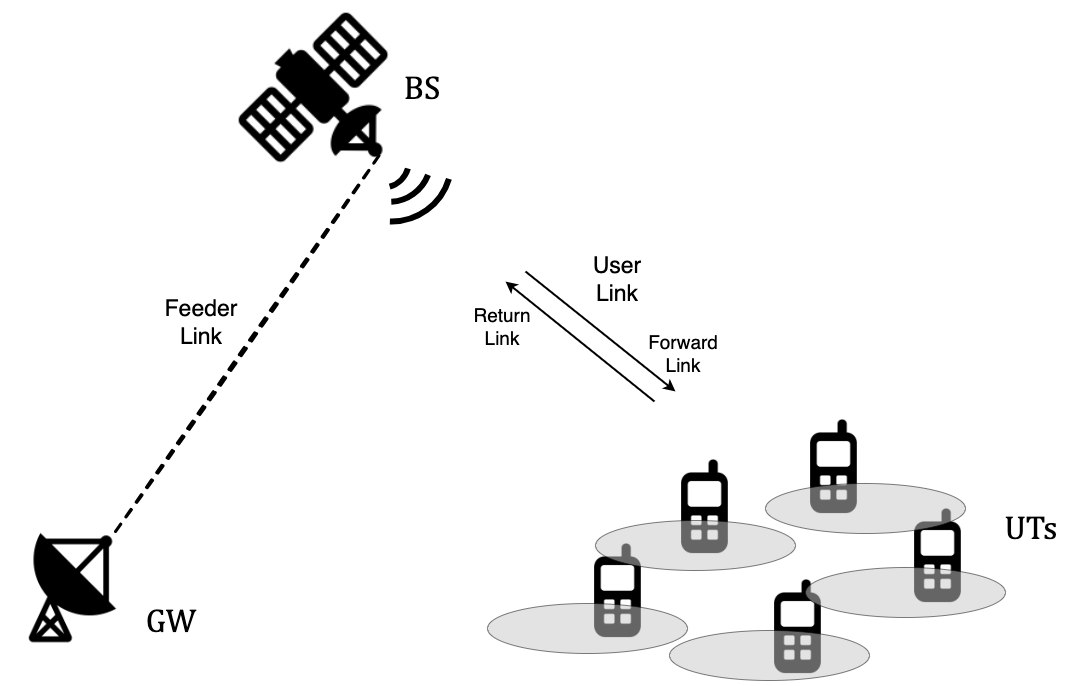
\includegraphics[width=0.8\textwidth]{figures/mobile_satellite_systems/05_hts_communication_systems/multibeam_satcom_annotated_big.png}
    \caption[Multibeam HTS communication system architecture]{Schematic view of the multibeam HTS communication system architecture.}
    \label{fig:multibeam_satellite_architecture}
\end{figure}

\subsection*{Features of Satellite Communications}
% --------------------------------------------------

% distinctive features of satellite communications
Compared to terrestrial \ac{MU}-\ac{MIMO} systems, satellite communications exhibit several distinctive features. 
The propagation conditions are dominated by a \acf{LoS} component between the satellite and the \acp{UT}, accompanied by a weaker scattered contribution arising from the local environment of the \ac{UT}~\cite{4_mimo_over_satellite_review}.
The free-space path loss is several orders of magnitude larger than in terrestrial links, and the received power can be further reduced by atmospheric impairments such as rain attenuation.
For mobile satellite services, however, communication often takes place in the L- or S-band, where propagation losses are smaller than in the Ka-band commonly used for fixed satellite services~\cite{1_signal_processing_for_satellites}.
This comes at the expense of a more limited available bandwidth, which further motivates aggressive frequency reuse.
For the present work, the two most relevant features are therefore the mobility of the \acp{UT} and the large propagation delay.

% mobility
The mobility of the \acp{UT} and/or the satellite makes the channel time-varying through Doppler effects.
For \ac{GEO} satellites, which appear essentially stationary relative to the Earth's surface, the satellite-induced Doppler shift is negligible, and the dominant source of channel variation is \ac{UT} motion alone.
For \ac{LEO} satellites, the high orbital velocity produces a substantial satellite-induced Doppler shift. 
However, since the satellite's trajectory is known with high accuracy, this contribution is deterministic and can be pre-compensated (see e.g.~\cite{doppler_compensation_mimo_leo}).
The residual, more difficult component to track is the Doppler shift induced by the motion of the \ac{UT}, since it depends on the instantaneous user velocity and propagation geometry.
So, in both cases, \ac{UT} mobility is the primary driver of channel time-variation, and it causes the channel to fluctuate at a rate governed by the \ac{UT} speed and the carrier frequency.

% popagation delay
The large geographical distances between the \ac{GW}, the satellite, and the \acp{UT} introduce a propagation delay that is several orders of magnitude larger than in terrestrial systems. 
For a \ac{GEO} satellite, which orbits at an altitude of approximately $35{,}786~\mathrm{km}$, the one-way propagation delay is on the order of $250~\mathrm{ms}$.
Even for a \ac{LEO} constellation, the \ac{RTT} remains in the tens of milliseconds.
Since the precoder is computed based on \ac{CSI} provided by the \acp{UT}, this delay implies that the channel used to design the precoder is inevitably outdated relative to the channel experienced when the precoded signal reaches the \acp{UT}.
In a static scenario, this mismatch is of limited importance.
In combination with a time-varying channel, however, it forms a major challenge for precoding design.

\subsection*{Channel Model}
% --------------------------

No single probabilistic model captures the full range of propagation conditions encountered in mobile satellite communications, and a variety of models have been proposed in the literature for different scenarios.

In this work, we begin with a deliberately simplified model in which the channel of \ac{UT}$_k$ is represented as a frequency-flat Rician fading channel~\cite{4_mimo_over_satellite_review, 7_coherence_time_non_terrestrial}:
\begin{equation}
\label{eq:rician_channel_model}
    \mathbf{H}_k(t) = \sqrt{\frac{\kappa}{\kappa+1}} \, \mathbf{H}_k^{\mathrm{LoS}}(t) + \sqrt{\frac{1}{\kappa+1}} \, \mathbf{H}_k^{\mathrm{NLoS}}(t),
\end{equation}
where $\kappa \geq 0$ is the Rician factor, $\mathbf{H}_k^{\mathrm{LoS}}(t)$ is the deterministic \acf{LoS} component, and $\mathbf{H}_k^{\mathrm{NLoS}}(t)$ is the time-varying stochastic \acf{NLoS} component.

The Rician factor quantifies the power ratio between the \ac{LoS} and the \ac{NLoS} contribution.
It typically takes values around $5~\mathrm{dB}$ in urban environments and up to $15~\mathrm{dB}$ or more in rural environments.
In this work, it is set to $5~\mathrm{dB}$.

The \ac{LoS} component is treated as time-invariant, and the small spatial variations across the antenna arrays are neglected. 
So, all entries of $\mathbf{H}_k^{\mathrm{LoS}}$ share a common, constant phase offset $\theta_k$ associated with \ac{UT} $k$:
\begin{equation}
\label{eq:rician_channel_LoS}
    \mathbf{H}_k^{\mathrm{LoS}} = e^{j\,\theta_k} \, \mathbf{1}_{N_R \times N_T}
\end{equation}
As a consequence, the \ac{LoS} component does not contain any temporal or spatial variation.

The \ac{NLoS} component $\mathbf{H}_k^{\mathrm{NLoS}}(t)$ captures the scattered multipath contribution.
Each entry is considered \ac{i.i.d.}, and modeled as a zero-mean unit-variance complex Gaussian random variable consistent with the Rayleigh fading model as described in Appendix~\ref{appendix:rayleigh_channel}. 
The temporal correlation of the \ac{NLoS} entries is governed by the Doppler spread induced by \ac{UT} mobility.
Under the classical isotropic scattering assumption, the power spectral density of each channel entry follows the Jakes model:
\begin{equation}
\label{eq:jakes_doppler_spectrum}
    S_{\mathbf{H}_k^{\mathrm{NLoS}}}(f) = \frac{1}{\pi f_D \sqrt{1 - (f/f_D)^2}}, \quad |f| \leq f_D,
\end{equation}
where $f_D = v f_c / c$ is the maximum Doppler frequency, determined by the \ac{UT} speed $v$, the carrier frequency $f_c$, and the speed of light $c$. 
Further details on the Doppler power spectrum are provided in Appendix~\ref{appendix_section:doppler_spectrum}, and the generation of a time-correlated random process with a prescribed autocorrelation function or power spectral density is addressed in Appendix~\ref{appendix:time_correlated_processes}.

The model as stated rests on two simplifying assumptions: spatial correlation between channel entries is neglected, and the \ac{LoS} Doppler shift is assumed to be perfectly pre-compensated.
While these assumptions yield a tractable and well-understood baseline, they do not always hold in practice.
At the end of the following chapter, we therefore describe how this model can be extended to a more realistic setting that accounts for spatial correlation and a residual \ac{LoS} Doppler component, and we briefly evaluate the impact of these features on the performance of the proposed precoding techniques.


\section{Classification}
\label{section:hts_classification}
% =============================================
%   Classification of Precoding Techniques
% =============================================

A large number of precoding techniques have been proposed for satellite communications, differing in the assumptions they make about the system and in the design objectives they pursue. A comprehensive survey can be found in~\cite{3_precoding_for_satellites_survey}. The objective of this section is not to reproduce this overview, but rather to position the present work within the broader landscape and to identify the techniques that are most closely related.

\subsection*{A Taxonomy of Precoding Techniques}
% --------------------------------------------

Besides the distinction between linear and nonlinear techniques, existing satellite precoding methods can be classified along several other non-exclusive axes. For each axis we briefly recall the main alternatives and indicate the choice made in this work.

A first distinction concerns the traffic model. In practical multibeam satellite systems, a single beam may simultaneously serve multiple \acp{UT} within the same frame, which leads naturally to a multi-group multicast formulation. 
To avoid additional complications introduced by multicast scheduling, we restrict the analysis to the unicast case, in which only a single \ac{UT} is served per beam.
A second axis concerns the optimization criterion. Depending on the system objective, the precoder may be designed to maximize the sum rate under a transmit power constraint, or to minimize the transmit power provided that \ac{QoS} metric is met.
Closely related to this is the choice of power constraint. In practical satellite payloads, each feed is typically driven by its own power amplifier, which makes per-feed power constraints the most natural formulation from an implementation perspective.
However, owing to the additional complexity associated with per-feed power constraints, most existing precoding techniques are formulated under a total transmit-power constraint.
In this dissertation, the emphasis is placed on sum-rate maximization subject to a total transmit power constraint, in line with the terrestrial \ac{MU}-\ac{MIMO} framework developed in the previous chapters.
A further classification axis is the system architecture. 
In large multibeam systems, precoding may be distributed across multiple \acp{GW}, and part of the processing may even be transferred on board the satellite in order to relax feeder-link limitations. 
Here, the simplest architecture is considered: a single \ac{GW} performs all precoding on the ground and serves the multibeam payload through a common feeder link.

Finally, and most importantly for the present work, precoding techniques differ in the type of \ac{CSI} assumed at the transmitter. 
Three regimes are commonly distinguished: perfect instantaneous \ac{CSI}, statistical \ac{CSI}, and imperfect or outdated \ac{CSI}. 
The vast majority of the satellite precoding literature assumes perfect instantaneous \ac{CSI} at the \ac{GW}.
This assumption becomes unrealistic in the scenario considered here, where the combination of large propagation delay and a time-varying channel due to a \ac{UT}-induced Doppler renders the \ac{CSI} available at the \ac{GW} systematically outdated.
Precoding under outdated \ac{CSI} is therefore the regime adopted in this work.

\subsection*{Related Work and Positioning}
\label{subsection:related_work_and_position}
% ------------------------------------------

To the best of our knowledge, only two works have addressed the design of linear precoding for mobile multi-beam satellite systems with outdated \ac{CSI} under assumptions comparable to ours.

The first is the work of Vázquez et al.~\cite{10_delayed_csi_precoding_for_satellites_spain}, which considers an L-band mobile interactive multi-beam system over a \ac{GEO} satellite. 
The authors model the feedback loop as a single delay $\tau$ on the order of $700$ milliseconds and adopt a simple closed-form \ac{MMSE} precoder.
Their key analytical observation is that, for a fixed precoder, the random phase fluctuations of the fading process affect the desired and the interfering terms symmetrically and therefore cancel in the resulting \ac{SINR}, only the amplitude fluctuations of the fading process remain visible. 
As a consequence, the ergodic sum rate is essentially unchanged by outdated \ac{CSI}, and the dominant practical impairment becomes the mismatch between the \ac{SINR} predicted by the outdated \ac{CSI} and the \ac{SINR} effectively experienced by the \acp{UT}, which is handled by fixed back-off margins in the link-adaptation stage.

The second is the work of Joroughi et al.~\cite{11_delayed_csi_precoding_for_satellite_luxembourg}, which considers a maritime multi-beam scenario at L-band. 
The channel is decomposed into a time-invariant beam-gain matrix and a time-varying diagonal attenuation matrix, and the authors propose two \ac{CSI} feedback strategies.
The first is a memoryless strategy that feeds the \ac{GW} with the latest delayed snapshot of the attenuation. The corresponding precoder is a conventional \ac{ZF} or \ac{MMSE} precoder computed from this estimate.
The second is a memory-based strategy that averages the attenuation over several past snapshots, and it is paired with a novel two-stage precoder: a first stage suppresses inter-beam interference, while a second diagonal stage compensates for the residual time-varying attenuation.

While the works above tackle the same regime of outdated \ac{CSI} in mobile multi-beam satellite systems, our approach differs in several aspects.
First, rather than focusing on a single precoder, we evaluate the impact of outdated \ac{CSI} on three different, commonly used linear precoders.
Second, instead of addressing the mismatch mainly through link-adaptation margins or temporal averaging and a dedicated robust precoder structure, we seek to compensate it in a more direct way.
